\documentclass[ngerman]{scrartcl}
\usepackage{babel}
\usepackage{csquotes}

% typography
\usepackage{fontspec}
\setmainfont{Open Sans}[
  BoldFont={Open Sans Bold},
  ItalicFont={Open Sans Italic}]
\setsansfont{Open Sans}[
  BoldFont={Open Sans Bold},
  ItalicFont={Open Sans Italic}]
\setmonofont{Menlo}
\usepackage[factor=2000]{microtype}

% graphics, drawings, etc.
\usepackage{xcolor}
\usepackage{graphicx}
\usepackage[most]{tcolorbox}
\usepackage{tikz}
\usetikzlibrary{shapes.geometric}
\usetikzlibrary{shapes.arrows}
\newtcolorbox{anmerkung}{%
  grow to left by=10pt,
  colback=black!10,
  colframe=white,
  coltitle=black,
  borderline west={4pt}{0pt}{black!30},
  boxrule=0pt,
  boxsep=0pt,
  %breakable,
  enhanced jigsaw,
  title={Anmerkung\par},
  fonttitle={\bfseries},
  attach title to upper={}}

% highlighting, lists, code
\usepackage{soul}
\usepackage{enumitem}
\usepackage{listings}
\lstset{
  basicstyle=\ttfamily,
  escapeinside=||,
  keywordstyle=\color{blue!50!black},
  stringstyle=\color{green!50!black}}

% nice tables
\usepackage{booktabs}
\newcommand{\tablespacing}[1]{\renewcommand{\arraystretch}{#1}}

% links
\usepackage[
  colorlinks,
  linkcolor={red!50!black},
  citecolor={blue!50!black},
  urlcolor={blue!80!black}
]{hyperref}

\title{Einführung in den Compilerbau}
\date{Wintersemester 2018-2019}
\author{Andreas Koch}

\begin{document}
  \maketitle
  \tableofcontents
  \newpage
  
  %\KOMAoptions{twocolumn}
  
  \section{Organisatorisches}
   
  \subsection{Grundlage der Vorlesung}
   
  Die Vorlesung basiert \hl{fast vollständig} auf \emph{Programming Language Processors in Java}\footnote{von David Watt und Deryck Brown, Prentice-Hall 2000}. Auszugsweise noch weiteres Material, z.\ B.\ zum ANTLR-Parsergenerator.
  
  \subsection{Übersichtswerk}
  
  Einen guten allgemeinen Überblick, aber im Detail mit anderen Schwerpunkten als diese Vorlesung, bietet \emph{Compilers, 2. Auflage}\footnote{Von Aho, Sethi, Ullmann, Lam, Addison-Wesley 2006. Auch auf Deutsch verfügbar.}.
   
  \subsection{Aufbau der Veranstaltung}
  
  Diese Veranstaltung ist logisch in mehrere Teile gegliedert.
  
  \begin{description}
    \item[Front-End\footnotemark] Übersicht, ca.\ 3 Wochen.
    \begin{itemize}
      \item Lexing und Parsing,
      \item Zwischendarstellungen.
    \end{itemize}
    \item[Middle-End] Übersicht, ca.\ 2 Wochen.
    \begin{itemize}
      \item Semantische- und Kontextanalyse.
    \end{itemize}
    \item[Back-End] Übersicht, ca.\ 4 Wochen.
    \begin{itemize}
      \item Laufzeitorganisation,
      \item Code-Erzeugung.
    \end{itemize}
    \item[Front-End-Generatoren] Verwendung, ca.\ 2--3 Wochen.
    \item[Java Virtuelle Maschine] ca.\ 1--2 Wochen.
  \end{description}
  \footnotetext{Die ersten drei Teile der Veranstaltung richten sich an die Veranstaltungen \emph{IMT3052} von Ivar Farup, Universität Grøvik, Norwegen; und \emph{Vertalerbouw} von Theu Ruys, Universität Twente, Niederlande.}
  
  \section{Einleitung}
  
  \subsection{Compiler}
  
  Ein Compiler ist eine Schnittstelle zwischen \emph{Mensch} und \emph{Maschine}. Er übersetzt von einer Programmiersprache (Menschenlesbar) in eine Maschinensprache (maschinenlesbar).
  
  \begin{description}
    \item[Programmiersprache] Gut für Menschen lesbar. Beispiele für Programmiersprachen sind:
    \begin{itemize}
      \item Smalltalk, 
      \item Java, 
      \item C++.
    \end{itemize}
    \item[Maschinensprache] Getrimmt auf
    \begin{itemize}
      \item Ausführungsgeschwindigkeit,
      \item Preis pro Chip, Fläche,
      \item Energieverbrauch,
      \item (nur selten) leichte Programmierbarkeit.
    \end{itemize}
  \end{description}
  
  \subsection{Auswirkung von Compilern}
  Mit den Eigenschaften entscheidet ein Compiler über die dem Nutzer zugängliche Rechenleistung. Durch gewisse Abwägungen kann ein Compiler ein Programm so kompilieren, dass es am schnellsten läuft oder dass der Resultierende Code an kleinsten ist.
  
  \begin{table*}[h]
  \centering
  \tablespacing{1.2}
  \begin{tabular}{@{}lp{.5cm}lp{.5cm}l@{}}
    \toprule
      Compiler && Ausführungszeit && Programmgröße\\
      \midrule
        GCC 3.3.6 && 7,5\,ms && 13\,KB\\
        ICC 9.0 && 6,5\,ms && 511\,KB\\
      \bottomrule
  \end{tabular}
  \caption{Bildkompression auf Dothan CPU, 2\,GHz}
  \end{table*}

  \subsection{Programmiersprachen}

\begin{description}
\item[Hohe Ebene] Smalltalk, Java, C++. Beispiel:
\begin{lstlisting}
let
  var i : Integer;
in
  i := i + 1;
\end{lstlisting}
\item[Mittlere Ebene] Assembly
\begin{lstlisting}
LOAD  |\hl{R1}|, (i)
LOADI |\hl{R2}|, 1
ADD   |\hl{R1}|, R1, R2
STORE R1, (i)
\end{lstlisting}
\item[Niedrige Ebene] Machinensprache
\begin{lstlisting}
01100001|\hl{00000110}|
0111001001000001
1011000100010010
10010001|\hl{00000110}|
\end{lstlisting}
\end{description}

\subsection{Abstraktionsebenen}

Auf den unteren Ebenen werden die Beschreibungen immer feiner, da man näher an der Zielmaschine (Hardware) arbeitet.

Der Compiler ist dafür zuständig, Details hinzuzufügen. In den obenstehenden Codebeispielen musste der Compiler unter anderem Register wählen, in denen die Werte währen dem Programmablauf zwischengespeichert werden. Außerdem musste die Adresse der Variable \verb|i|, hinzugefügt werden, wobei hier \verb|00000110| verwendet wurde.

Diese Details werden mithilfe von verschiedensten Algorithmen ergänzt, welche die \hl{Programmeigeschaften Analysieren} und durch die \hl{Synthese von Details} die Beschreibung Verfeinern.

\section{Zielmaschine}

\subsection{Auswirkungen der Zielmaschine}

\begin{figure}\label{fig:dlx}
\includegraphics[width=\textwidth]{media/dlx}
\caption{Die DLX RISC Prozessorarchitektur}
\end{figure}
\begin{figure}
\includegraphics[width=\textwidth]{media/tigersharc}
\caption{Analog Devices TigerSHARC}\label{fig:tigersharc}
\end{figure}
\begin{figure}
\caption{Ein \emph{Synergistic Processing Element} eines Cell Prozessors.}\label{fig:spe}
\end{figure}
% TODO figure.

Die Zielmaschine hat einen Einfluss auf die Architektur des Compilers. So basiert zum Beispiel die DLX Architektur von John Hennessy und David Patterson auf der MIPS Architektur, und ist nur leicht verändert um diese zu modernisieren. Damit ist es sehr einfach, einen Compiler zu bauen, der für diese Architektur Code generiert.

Etwas komplizierter wird es mit der \emph{TigerSHARC} Architektur von Analog Devices. Dies ist ein Beispiel für ein DSP, also \emph{Digital Signalling Processor}. Es gibt hier zwei \emph{Computational Blocks}, damit parallel Rechnungen ausgeführt werden können. Diese können aber nicht kommunizieren, also muss der Compiler drauf achten, dass auf die Register nur von dem jeweiligen Block aus zugegriffen werden können. Außerdem besitzt diese Architektur separate Rechenblocks, um Adressen zu bestimmen. Ein Compiler für diese Architektur muss also wissen, wie die Architektur aufgebaut ist, um sie effizient zu nutzen.

Am problematischsten wird das aber erst bei extremen Architekturen wie der des IBM/Sony \emph{Cell} Prozessors. Hierbei handelt es sich um eine sehr gewagte, und wie sich leider herausgestellt hat, zu komplexe Architektur. Es gibt ein PowerPC-basierten Hauptprozessor, der aber nicht sehr leistungsstark ist. Die eigentliche Arbeit kann von \emph{Synergistic Processing Elements}, kurz SPE, ausgeführt werden. Diese sind so konstruiert, dass ein sorgfältig produzierter Instruktionsstream die Hardware maximal ausnutzen kann, mit parallelen Arithmetischen- und Speichereinheiten (siehe Abbildung \ref{fig:spe}).

\subsection{Anforderungen an CPUs}

Je nach Anwendungsgebiet sind die Anforderungen mehr oder weniger wichtig. 
\begin{itemize}
  \item Rechenleistung
  \item Datentype (Gleitkomma, ganzzalig, Vektoren)
  \item Operationen (Multiplikationen, MAC\footnote{Mir als \emph{fused multiply and add} bekannt, eine Operation, die vor allem für Matrizenmultiplikation signifikant ist.})
  \item Speicherbandbreite (parallele Speicherzugriffe)
  \item Energieeffizienz
  \item Platzbedarf (für den Prozessorchip)
\end{itemize}
Oft können manche Anforderungen nur durch spezialisierte Prozessoren erfüllt werden.

\subsection{Paralleles Rechnen}

Paralleles Rechnen ist die Königsklasse der Forschung. Warum eigentlich? Das Wettrennen der Taktfrequenzen ist im großen und ganzen vorbei, mehr als \textasciitilde4\,GHz ist nicht realistisch. Also ist \hl{der Trend weg von hochgetakteten Einzelprozessoren und hin zu vielen (2-8, teilweise 16) Prozessoren}, die aber weniger schnell getaktet werden. Dadurch erreicht man mehr Rechenleistung. Aber wie kann man für solche parallele Rechenkapazitäten programmieren?

Erste praktische Ansätze sind OpenMP, mit dem man für parallele CPUs programmieren kann. {OpenCL} kann mit heterogenen Systemen (GPUs, CPUs, experimentell auch FPGAs) arbeiten, und für NVidia Grafikkarten gibt es {CUDA}. \hl{Diese Lösungen erfordern aber aktuell noch, dass der Programmierer explizit für ein paralleles System programmiert. Es gibt noch keine automatische Parallelisierung}.

\subsection{Compilerbau in der Lehre}

Warum wird der Compilerbau so früh gelehrt? Es handelt sich hierbei um eine Kombination von verschiedenen Disziplinen. Zum Compilerbau benötigt man einen \emph{Parser}, welcher zur theoretischen Informatik gehört. Man braucht auch das Hintergrundwissen der \emph{Architektur der Zielmaschine}, welches zur technischen Informatik gehört. Außerdem braucht man zum Compilerbau Kenntnisse von Software-Engineering, was zur praktischen Informatik gehört. Damit vereint der Compilerbau drei wichtige Disziplinen.

\section{Aufbau}

\subsection{Vorgehen}

Compiler arbeiten generell in mehreren Phasen. In Abbildung \ref{fig:compilerstages} sind diese Phasen aufgezeigt. Außerdem sind die  Zwischendarstellungen, die zum Informationsaustausch zwischen den Phasen genutzt werden, dargestellt.

\begin{figure}\centering
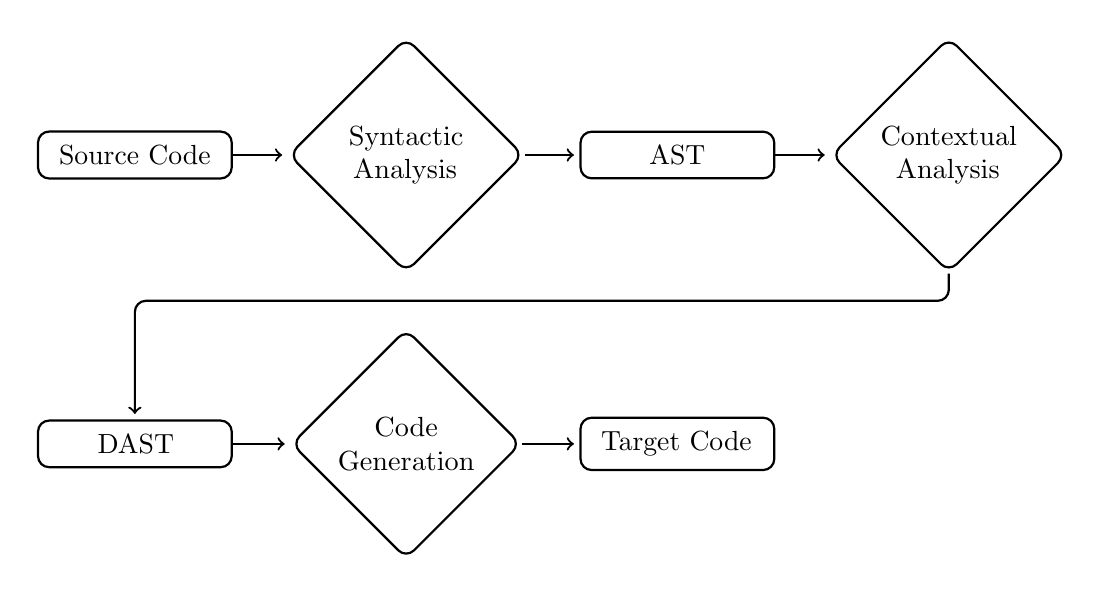
\begin{tikzpicture}[
  stage/.style={diamond, draw=black, thick, text width=6em, text centered, inner sep=0.1em, rounded corners},
  repr/.style={rectangle, draw=black, thick, text width=6em, text badly centered, inner sep=0.5em, rounded corners},
  line/.style={draw, thick, ->, shorten >=2pt, rounded corners}]
\matrix[column sep=2em, row sep=1em]{
  \node[repr] (source) {Source Code};
  & \node[stage] (syntax) {Syntactic Analysis};
  & \node[repr] (ast) {AST};
  & \node[stage] (context) {Contextual Analysis};\\
  \coordinate (phantoml);
  &&& \coordinate (phantomr);\\
  \node[repr] (dast) {DAST};
  & \node[stage] (generation) {Code Generation};
  & \node[repr] (target) {Target Code};
  &\\
};
\begin{scope} [every path/.style=line]
\path (source) -- (syntax);
\path (syntax) -- (ast);
\path (ast) -- (context);
\path (context) -- (phantomr) -- (phantoml) -- (dast);
\path (dast) -- (generation);
\path (generation) -- (target);
\end{scope}
\end{tikzpicture}
\caption{Zwischendarstellungen für den Informationsaustausch}\label{fig:compilerstages}
\end{figure}

\subsection{Syntaxanalyse}

Bei der Syntaxanalyse wird überprüft, ob das Programm Syntaxgerecht aufgebaut ist. 

\subsection{Kontextanalyse}

Bei der Kontextanalyse werden Variablen ihren Deklarationen zugeordnet. Ausßerdem werden die Typen von Ausdrücken berechnet.

% TODO graphics, text.

\subsection{Code-Erzeugung}

Wenn das Programm syntaktisch und kontextuell korrekt ist, kann es in die Zielsprache übersetzt werden. Eine Zielsprache kann eine Low-Level Sprache wie die Maschinensprache oder Assembly, aber auch C oder eine andere Hochsprache.

Dazu wird DAST-Teilen Instruktionen der Zielsprache zugeordnet. Variablen werden gehandhabt, indem zum Beispiel bei einer Deklaration Speicherplatz reserviert wird, und bei der Verwendung der zugeordnete Speicherplatz referenziert wird.

\section{Optimierung}

\subsection{Optimierender Compiler}

% TODO graphic

Bei einem optimierenden Compiler findet die Kompilierung in drei Phasen statt.

\begin{description}
\item[Front-End] Macht die syntaktische und kontextuelle Analyse und gibt den AST in einem IR-Format (\emph{Intermediate Representation}) aus.
\item[Back-End] Liest das IR, und erzeugt den Code.
\item[Middle-End] Transformation von Zwischendarstellungen. Dieses arbeitet auf der IR. Hier wird kein Code ausgegeben, sondern nur der IR optimiert. Intern werden hier auch oft zusätzliche Darstellungen verwendet werden.
\end{description}

\begin{anmerkung}
LLVM ist ein sehr bekanntes Projekt, welches eine Art Plugin-basierte Architektur aufweist. Es können Front-Ends geschrieben werden, die unterschiedliche Programmiersprachen unterstützen (zum Beispiel \verb|clang| für C und C++, \verb|rubinius| für Ruby). Optimierungen können ebenso als Plugin geschrieben werden, und arbeiten auf dem LLVM IR. Es können außerdem Back-Ends geschrieben werden, die für unterschiedlichste Architekturen Code ausgeben. Somit funktioniert zum Beispiel das \emph{Emscripten} Projekt, mit welchem man C und C++ Code in JavaScript kompilieren kann.
\end{anmerkung}

\subsection{Beispiele für Optimierung}

\begin{description}
\item[Constant Folding] Bei dieser Optimierung werden Ausdrücke, die ein konstantes Ergebnis haben, von Optimierer ausgewertet. Hat man zum Beispiel den Code
\begin{lstlisting}[language=C]
int x = (2 + 3) * y;
\end{lstlisting}
Bei dem Constant Folding erkennt der Compiler, dass der ausdruck \verb|2 + 3| konstant ist. Er kann den Ausdruck dann bestimmen, und den Code in eine minimierte Version transformieren.
\begin{lstlisting}[language=C]
int x = 5 * y;
\end{lstlisting}
\begin{anmerkung}
Sowohl C++ (seit C++11) als auch Rust haben mittlerweile Support für Constant Folding in die Sprache eingebaut. Mit dem \verb|constexpr| Keyword kann man dem Compiler sagen, dass er einen Funktion oder Variable als Konstante ansehen und diese während der Kompilierung auswerten soll.
\end{anmerkung}
\item[Common Subexpression Elimination] Hierbei werden Ausdrücke (\emph{Subexpressions}), die öfters im Code vorkomment (\emph{Common}) eliminiert. Hat man zum Beispiel folgenden Code:
\begin{lstlisting}[language=C]
int x = 5 * a + b;
int y = 5 * a + c;
\end{lstlisting}
So kann der Compiler erkennen, dass der Ausdruck \verb|5 * a| mehrmals vorkommt. Wenn er garantieren kann, dass der Wert von \verb|a| während den Instruktionen konstant bleibt, kann er diese vereinfachen, indem er eine temporäre Variable einführt.
\begin{lstlisting}[language=C]
int _temp = 5 * a
int x = _temp + b;
int y = _temp + c;
\end{lstlisting}
\end{description}

% TODO more

\section{Syntax}

\subsection{Syntax oder Grammatik}

Der Syntax beschreibt die Satzstruktur von korrekten Programmen. Jede Sprache hat ihren eigenen Syntax. So ist zum Beispiel der folgende Ausdruck Syntaktisch korrekt in C.
\begin{lstlisting}[language=C]
int n = m + 1;
\end{lstlisting}
Der Satz \enquote{Ein Kreis hat zwei Ecken} ist wiederum eine syntaktisch korrekte Aussage im Deutschen (was aber nicht bedeutet, dass diese auch \emph{semantisch} korrekt ist).

\subsection{Kontextuelle Einschränkungen}

Nicht jede Aussage, die syntaktisch korrekt ist, ist in dem Kontext auch erlaubt. Es gibt gewisse Regeln, die vom Geltungsbereich (\emph{scope}) und dem Typ von Aussagen abhängen. So ist der folgende Code zum Beispiel nur dann korrekt, wenn die Variable \verb|x| deklariert ist.
\begin{lstlisting}[language=C]
int y = 2 * x;
\end{lstlisting}
Bei dem Satz \enquote{Ein Kreis hat zwei Ecken} ist der Fehler, dass ein Kreis keine Ecken besitzt. Hier passen die Typen nicht, ein Objekt der klasse \emph{eckige Geometrische Formen}, wie zum Beispiel das Dreieck, würde hier kontextuell passen (aber der Satz wäre dann semantisch immer noch falsch).

\subsection{Semantik}



\end{document}










